%% Background Theory
%%=========================================

\chapter{Background Theory}
\label{ch:background}
In this chapter we will look at relevant theory and the underlying structure of our problem.

%%=========================================

\section{Understanding Our Problem}
Understanding what type of problem we are trying to solve is important. While many problems may seem similar in nature, small factors can influence how a problem is best solved. Some factors even influence the problem so much that it becomes a completely different one. This chapter investigates what type of problem we are trying to solve.

The next section evaluates what data we want to give to our model, and what results we hope the model outputs. Section \ref{sec:classification_explanation} presents the concept of classification, and section \ref{sec:classification_similarities_and_dissimilarities} explains how our problem is different from it.

%%=========================================

\section{Evaluating Problem Input and Output}
In our particular problem we have a input that is a matrix or a vector of binary data. The binary input denotes the color of a particular pixel at the given location in our ``signature". We want the output to be what character(s) the matrix or vector is made out of. For example, if our characters are the upper cased letters in the English language, we could want our output to be in the range 1 to 26, denoting A to Z. See \ref{eq:input_output_example} for example input and output for the word ``ALLIED".

\begin{equation}
    \label{eq:input_output_example}
    \begin{aligned}
       \vec{rawInput}        &= \lbrack 4W, 3B, 7W, 3B, 8W, 3B, 18W, 3B, 23W, 3B, 13W, 14B, 6W, 3B, 10W, 3B \rbrack \\
       \vec{encodedInput}    &= \lbrack 2, 1, 3, 1, 4, 1, 5, 1, 6, 1, 7, 8, 9, 1, 10, 1 \rbrack \\
       \vec{output}          &= \lbrack 1, 12, 12, 9, 5, 4 \rbrack \\
       word                  &= \text{ALLIED}
    \end{aligned}
\end{equation}

Note that in example \ref{eq:input_output_example} we encoded our input to whole integers. The encoding is done by assigning unique numbers to each input value. In our case, we assigned numbers ranked by frequency. `3B` occurs seven times in the raw output, while all the other values have a frequency of one.

\subsection{Input Format}
Our input has the feature that they form a sequence. Both the values in the sequence, and the ordering of the sequence is crucial for prediction. This is fundamentally different from other problems such as traditional image recognition, where the exact location of a pattern is not important.

Because the input forms a sequence, it is important that the entire sequence is read, and that we do not cut the sequence off at the end, removing important information that we need. We do also lack the concept of ``stop words" in our problem. Nowhere in our sequence is a special value used that indicates that one character ends and another begins. Using a stop word would make the problem easier to solve, as we would know in what area each character could be found. Instead of relying on stop words, we want our model to find a pattern in the sequence data that makes sense. This pattern, if correctly predicted, would have ``invisible" stop words at the correct places in the original input, without having been explicit stated.

\red{Add more}

\subsection{Output Format}
As with the input, our output also form a sequence. Both the values in the sequence, and the ordering of the sequence, is important. The words `HELLO` and `HLLOE` contains the same letters, but have a different meanings. Understanding that both the individual values in the output sequence, as well as the placement of each of them, is important for understanding how our problem is different from many others. The structure of the output is elaborated more in section xx.

%%=========================================

\section{Classification}
\label{sec:classification_explanation}
Classification has two distinct meanings. Classification with supervised learning we know for a fact how many classes exists, and our goal is to find a rule that can be used to classify an observation in one or more of these classes. Classification with unsupervised learning is often called clustering. This is the task of given a set of unlabeled data, we want to find the existence of classes or clusters in the data. In our particular problem, we know the labels for our observations, so our problem falls in the task of supervised learning.

The goal of classification is, as previously stated, to create a function that can be take an observation and give it one or more classes. The classifier is ``trained" on a set of data where we know the correct labels for each of the observations. With this training, the classifier should be able to ``learn" how to do classifications on its own. The important factor here is that the classifier should not just ``remember" earlier observations and simply return the correct answers, it should learn how to calculate the answers instead. 

\begin{equation}
    \label{eq:key_value_map}
    h: K \mapsto V
\end{equation}

In \ref{eq:key_value_map} $K$ denotes the keys, and $V$ denotes the values, our input and output respectfully. \ref{eq:key_value_map} is a simple look up, similar to how data structures such as hash maps. Unless the key $k$ has an exact match in $K$, it has no way of returning any value. Instead of the look up in \ref{eq:key_value_map}, we want a function as in \ref{eq:simple_function}, where the function $f(x)$ does some calculation to derive at the result $y$.

\begin{equation}
    \label{eq:simple_function}
    f(x) = y
\end{equation}

\subsection{Example of Classification}
\label{sec:classification-example}
Image classification is a common example of classification. A model is given the image data, and a set of categories, and its job is to identify in which category, or categories, the image belongs.

Figure \ref{fig:facebook-classification-example} illustrates classification using computer vision software. It contains an photo of Hovedbygget at Gløshaugen. The photo was uploaded to Facebook, and classified by their computer vision software. Using the Show Facebook Computer Vision Tags Chrome extension\footnote{\url{https://github.com/ageitgey/show-facebook-computer-vision-tags}}, we can see the categories in the top right corner of the photo.

\begin{figure}[H]
    \label{fig:facebook-classification-example}
    \centering
    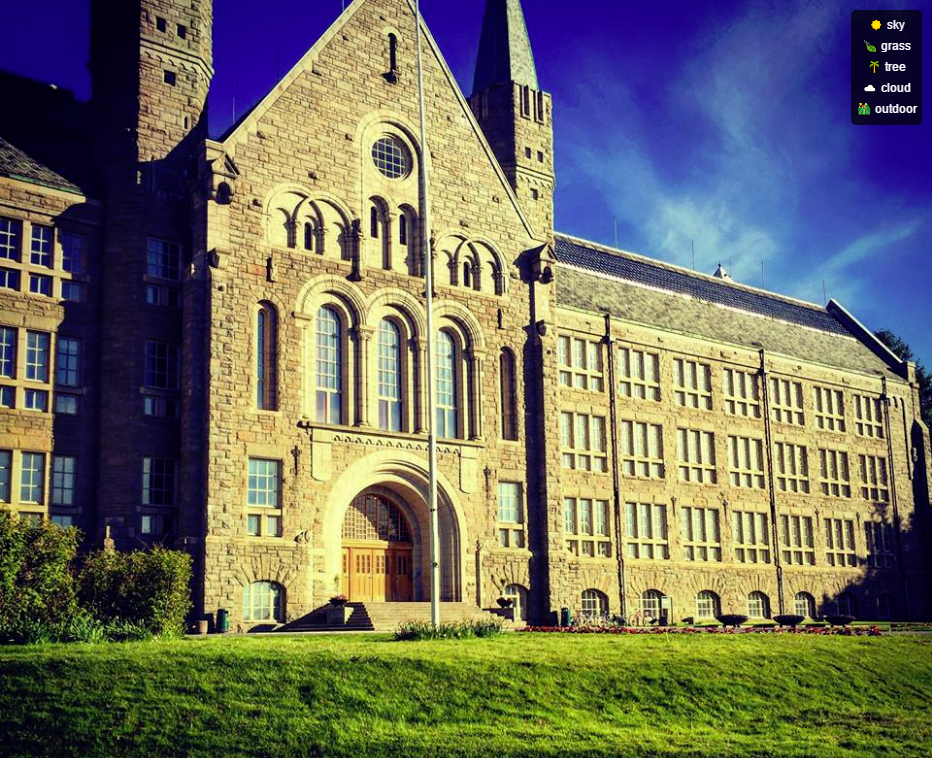
\includegraphics[width=0.7\textwidth]{fig/chapter4/facebook_classification_example.jpg}
    \caption{Personal photo of Hovedbygget, classified by Facebook}
\end{figure}

When Facebook classified my image, their software took all the categories they have, and gave each of them a probability based on what the software had seen in their training set. All the categories above a given threshold were returned and assigned to my image. 

\subsection{Dissimilarities}
To understand our problem behaves, dissimilarities to typical classification is presented to illustrate this.

\subsubsection{Meaning of Output}
As illustrated with the image classification of Figure \ref{fig:facebook-classification-example} in section \ref{sec:classification-example}, typical classification algorithms does not return the output the way we need in our problem. As already stated, the classifier in this case returned all the classes above a given threshold given its probability based on earlier observations in its training set. While the categories can be sorted by their probability, there is no other notion of ordering among them. See algorithm \ref{alg:classification_probability_example}, that illustrates how the output is handled in a model like this. The algorithm inputs a list of probabilities, which in this case would be the probabilities given to each category by the classifier, and outputs a list of tuples consisting of the probabilities and their index values for categories above a given threshold.

In our problem the ordering is, as already emphasised, crucial. Words are not the same when their letters are reordered. While we could look at the entire output vector as a single category, but that would require one category for each word, making it not only very insufficient, but would also make it impossible to classify new, unseen words.

\begin{algorithm}
    \caption{Return classified categories with probabilities and indexes above a given threshold
        \label{alg:classification_probability_example}}
    \begin{algorithmic}[1]
        \Statex
        \Function{return\_categories}{$X, t$}
            \Let{$res$}{$[ ]$} \Comment{Initialize empty list}
            \For{$i \gets 1 \textrm{ to } X.length$}
                \If{$X[i] \ge t$}
                    \Let{$res$}{$(X[i], i)$} \Comment{Add tuple (probability, index) to list}
                \EndIf
            \EndFor
        \State \Return{$res$}
        \EndFunction
    \end{algorithmic}
\end{algorithm}

%%=========================================

\section{Sequence Classification}
Sequence classification is a type of problem that falls in the general task of classification as presented in section xx. This particular problem however, has a characteristic that makes it more specialized than many other classification tasks.

The characteristics lies in how the classifier interprets the input. As we have emphasized before, out input is a sequence of values. Image classification is often called contextual, which means that the classification is based on the relationship between nearby data. For image classification, this makes sense as a single pixel itself does not make much sense, but given a group of pixels, we can try to recognize certain traits or patterns. In sequence classification, we must evaluate the entire sequence as a whole. Considering just the nearby values would not be sufficient in trying to make sense of a input sequence. \red{Images are dense, text is sparse}

A typical sequence classification example is classification of reviews and an associated score, which can be either a number, or a positive/negative value. The reviews contains the text from the reviewer, which will typically contain either positive or negative worded words. Table \ref{table:sequence-classification-illustration} contains an illustrative reviews. The importance of interpret the input as a whole makes sense when you consider that ``best restaurant" and ``best to avoid this restaurant" contains some of the same words, but the meaning is opposite.

\begin{table}[ht]
    \centering
    \begin{tabular}{|l|l|}
        \hline 
        \textbf{Review}                                  & \textbf{Recommends} \\ \hline
        The food tasted terrible and the place was dirty & No                  \\ \hline
        Food was expensive, and the waiter was lazy      & No                  \\ \hline
        Best restaurant I ever ate at.                   & Yes                 \\ \hline
    \end{tabular}
    \label{table:sequence-classification-illustration}
    \caption{Illustrative review data}
\end{table}

As with image classification, sequence classification outputs the categories and their respective probabilities. 

%%=========================================

\section{Sequence Labeling}
Sequence labeling is a different type of problem from statistical classification. Where statistical classification gave input a set of labels based on probability calculated from the overall input, sequence classification gives each input value a label. Also different from classification tasks is that sequence labeling does not have feature vectors.

"Different from
the classification task on feature vectors, sequences do not
have explicit features."

https://www.cs.sfu.ca/~jpei/publications/Sequence%20Classification.pdf

\subsection{Natural Language Processing}
Natural Language Processing is a sequence labeling task. In NLP we want to analyze an input, and 

%%=========================================

\section{Sequence Prediction}

%%=========================================

\section{Sequence to Sequence Learning}
Sequence to sequence learning is yet another type of machine learning that falls outside the typical classification tasks. In sequence to sequence learning, the input sequence is evaluated, and the output is another sequence. The task of the model is to find patterns in the input sequence that returns the corresponding output sequence. Different from the other approaches and tasks explained this far, the 

\begin{equation}
    \begin{aligned}
        f(\vec{input}) = \vec{output}
    \end{aligned}
\end{equation}